\chapter{Machine Learning Models}
\label{chapter:MLM}
Machine learning is a scientific discipline focused on the development of
algorithms based on learning from examples. This idea has become central to the
design of search engines, robots systems and forecasts applications that process
large data sets. Usually machines designed to forecast financial time series
requires long training period and therefore they are not suitable to be updated
with stream data. Online machine learning techniques tackle this problem by
updating the model with new data or by computing a new model considering less data so
they can give a response in a short period of time.

\vspace{0.5cm} 

\section{Introduction}
Machine Learning (ML) studies computer algorithms for learning patterns to complete a task, to make accurate predictions or to behave intelligently. The
learning is always based on samples and the objective is about to do better in
the future based on the past experiences in an automatic way. ML is a sub-area
of artificial intelligence and broadly intersects with other fields such as
statistics, mathematics, physics and computer science.  There are many examples
of machine learning problems: time series forecasting, image processing, face
detection, spam filtering, weather prediction, search engines, among many
others.

ML models are often more accurate than what can be created through direct
programming. The reason for this is that ML models are data driven and are able
to examine large amounts of data.

There are three types of ML classified depending on the nature of the learning
input or output available to a learning system:

\begin{description}
\item[Supervised learning]  the input data is a tuple which contains the example
input and its desired outputs (also called labels). The list of tuples is called
the training set. The concept of supervised learning comes from the supervisor,
acting as a teacher in the learning process. The goal is to learn a general rule
that maps inputs to outputs optimising a target function. There are two related
problem types in supervised learning: classification and regression problems
\cite{bishop2006}. Its two mainstream approaches are: support vector machines
(SVMs) \cite{vapnik1998} and ensemble learning \cite{breiman1998}. Furthermore,
supervised learning can be categorised into offline or batch learning and online
learning (see section~\ref{sec:onoffline}). 
\item[Unsupervised learning] also known as clustering \cite{ben2005}. In this
type of learning no labels are given and the system has to find a structure on
its own, discovering hidden patterns in data.
\item[Reinforcement learning] is the problem faced by an agent that must learn
through trial-and-error interactions with a dynamic environment. It is based on
programming agents by reward and punishment without the need to specify how the
task is to be achieved \cite{sutton1998}.
\end{description}


\section{Statistical learning theory} \label{sec:mltheory}

All ML problems can be viewed as optimisation problems. The ML core task is to
define a learning criterion, i.e the function to be optimised. 

Supervised learning is most popular and most commonly used in modelling
financial problems and the assessments of this method and their results in
practice are fairly good. Therefore, in this thesis we will adhere to this trend
and we will use supervised learning.

The basic setting for supervised learning is a {\em data set\/} $X$, 
and an  {\em outcome set\/} $Y$.
For our purposes $X$ will be $\R^m$, $m\in\N$, and $Y$ either $\R$
in the case of regression problems, or $\{-1,1\}$ in the case of
classification problems.
In addition we have a plurality of {\em training sets\/}
$$
S=\bigg\{ (\mathbf{x}_k,y_k)\in X\times Y \mid k=1,\dots,n \bigg\}
\subseteq X\times Y\,,
$$
where the members of $S$ have been drawn randomly and independently
from $X\times Y$ according to an {\em unknown\/} joint distribution
function $p(\mathbf{x},y)$ on $X\times Y$.
We gather all these training sets in a subset $\mathscr{T}$ of
$\mathscr{P}(X\times Y)$.

In addition, there is a {\em learning algorithm\/} $\mathcal{A}$ that
associates to every data set one and only one learning function
$f\in\mathscr{H}$.
Thus $\mathcal{A}$ can be considered as a function:
$$
\mathcal{A}:\mathscr{T}\to\mathscr{H}\,,\qquad
S\mapsto\mathcal{A}(S)=f\quad\forall S\in\mathscr{T}\,.
$$ 

{\em Supervised learning\/} consists then in finding a {\em learning function\/}
$f:X\to Y$ that minimise the expected error of the loss function $V(f(\mathbf{x}),y): Y
\times Y$ defined as:

\begin{equation}\label{eq:lossfunction}
V(f(\cdot),\cdot):X\times Y\to\R_0^+\,,\qquad
(\bfx,y)\mapsto V\big(f(\bfx),y\big)
\end{equation}

\noindent where $V(f(\mathbf{x}),y)$ denote the price paid for mistakes, $f:X=\R^m\to Y$
and $y=f(\mathbf{x})\in\R$. Therefore, $V(f(\mathbf{x}),y)=0$ if $\;f(\mathbf{x})=y$.

Given a function $f$ a loss function $V$ and a probability distribution $p$ over
$X \times Y$, the expected error of $f$ is:

\begin{equation}
\label{eq:expetedrisk}
E\big[ V( f(\cdot),\cdot) \big]
= \int_{X\times Y} V\big( f(\mathbf{x},y) \big)\,dp(\mathbf{x},y)\,.
\end{equation}


For regression, the most common loss function is square loss or $L_{2}$ loss function:
\begin{equation}
\label{eq:l2loss}
V(f(\mathbf{x}),y) = (f(\mathbf{x})-y)^2
\end{equation}
\noindent another option is the L1 loss
\begin{equation}
\label{eq:l1loss}
V(f(\mathbf{x}),y) = |f(\mathbf{x})-y| \, .
\end{equation}
\noindent the choice of loss function here gives rise to several well-known
learning algorithms such as regularised least squares and support vector
machines. %verificar esto

Since the true distribution is unknown and only training samples are available,
the objective is to estimate a function $\widehat{f}$ through empirical risk
(training error) minimisation (ERM): 

\begin{equation*}
\widehat{f} = \argmin_{f \in \mathscr{H}} R_{\text{emp}}[f] 
\end{equation*}

\noindent where, 

\begin{equation} 
\label{eq:erm}
R_{\text{emp}}[f] = \frac{1}{n} \sum_{i=1}^n V(f(x_i),y_i)   
\end{equation}

The ERM is a Riemann sum approximation of the expected error of $f$ shown in
equation~\eqref{eq:expetedrisk}. By the law of large numbers it is known that:

\begin{equation}
\frac1n\,\sum_{i=1}^n V\big( f(\bfx_i,y_i) \big)
\overset{n\to\infty}{\longrightarrow} E\big[ V(f(\cdot),\cdot)\big]\,.
\end{equation}


\subsection{Learning algorithms}
In all learning algorithms that are trained from example data, there is a
tradeoff between three factors \cite{dietterich2003}:
\begin{description}
\item[Complexity or capacity of the hypothesis class] is defined in terms of the
Vapnik-Chervonenkis (VC) dimension, which corresponds to the number of training
points that can be classified exactly by the hypothesis space. More formally,
the VC dimension of the hypothesis space $\mathscr{H}$ defined over instance
space $X$ is the size of the largest finite subset of $X$ shattered by
$\mathscr{H}$. The dataset $S$ is shattered by hypothesis space $\mathscr{H}$ if
and only if for every dichotomy of $S$ there exists some hypothesis in
$\mathscr{H}$ consistent with this dichotomy. A dichotomy of a set $S$ is a
partition of $S$ into two disjoint subsets \cite{vapnik2013nature}.

For example, the VC dimension of the lines in the plane is explained in figure
\ref{fig:vcdimension}:


\begin{figure}[!h]
  \centering
  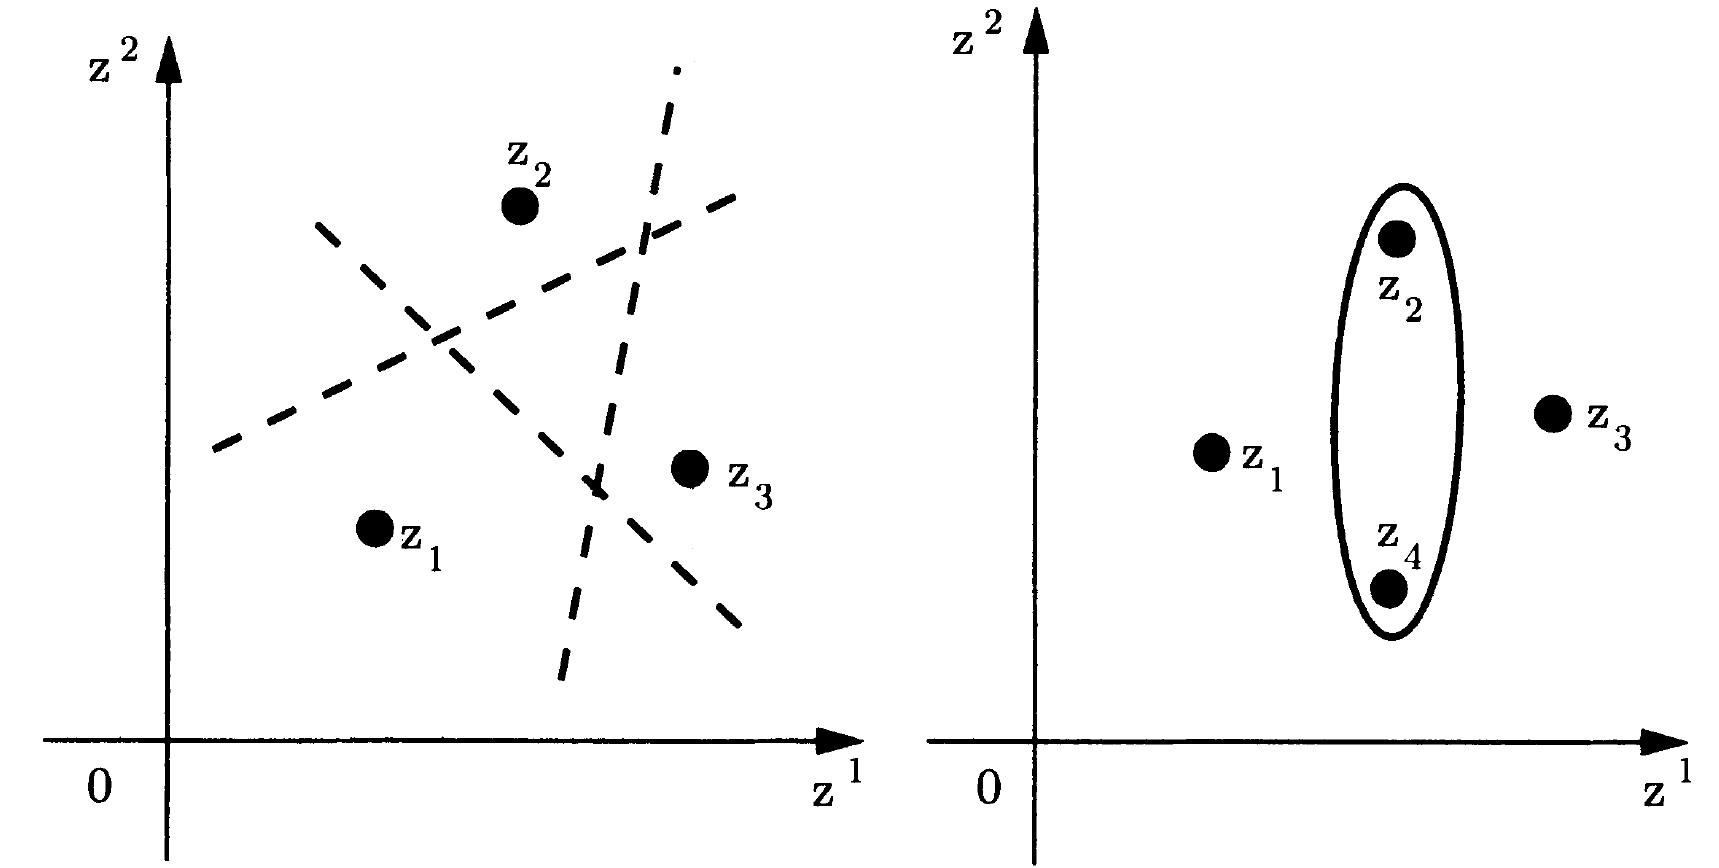
\includegraphics[width=0.8\textwidth]{img/VCdimension}
  \caption[VC dimension example]{VC dimension example from \cite{vapnik2013nature}. The example shows 2-dimensional vectors $z_k=(x_k,y_k)$,  $k=1,2,3,4$. The left figure
  shows that the 3 dichotomies can be shattered by a line in a plane. However, if we
  add an extra vector $z_4$, it is impossible to shatter them with a
  line. Therefore, linear classifiers has VC dimension equals to $d+1$ where $d$
  is the dimension of the instance space $X$.}
  \label{fig:vcdimension}
\end{figure}

A key point is Radon's theorem in discrete geometry \cite{peterson1972geometry}
($\text{co}(A)$ denotes the convex hull of $A$):

\begin{theorem}[J. Radon]
Let $S\subset\R^d$ be a subset containing at least $d+2$ elements. 
Then there exist {\bf disjoint} subsets $A\subset S$ and $B\subset S$
such that
$$
\text{co}(A)\cap\text{co}(B)\neq\emptyset
$$
\end{theorem}

Radon's theorem implies that in $\R^d$ any set of $d+2$ or more vectors has at least one dichotomy which cannot be
separated (shattered) by any plane in $\R^d$. Thus the VC-dimension in $\R^d$ cannot be greater than $d+1$.



\item[Generalisation accuracy on new examples] is the capability of the
algorithm to generate the right output for an input instance outside the
training set. It is measured by the expected risk (equation~\eqref{eq:expetedrisk}).
\item[The amount of training data] in most cases, generalisation accuracy
increases as the amount of training data increases.
\end{description}


The relationship between generalisation error and the amount of training or
input data is intuitive: the more data is given to the learning model $f$, the
more evidence the algorithm has about the problem. In the limit, the input data
will contain every possible example, so the algorithm will generalize perfectly.
However, for some $f \in \mathscr{H}$, the best hypothesis $\hat{f}$ might be far away to
the best hypothesis class but it is the best that all the learners can hope.
Therefore, to choose the right hypothesis class $\mathscr{H}$ is crucial. The error of
this best hypothesis is formalised as the {\em approximation or generalisation
error} \cite{niyogi1996relationship}.

Additionally, we do not have infinite data but only some finite random sample
set to find an hypothesis, the additional error caused by finiteness of the
data, is called {\em estimation error}. The amount of data needed to ensure a
small {\em estimation error} is referred to as {\em sample complexity} of the
problem.

The relationship between the generalisation error and the hypothesis complexity
is less intuitive. If the class $\mathscr{H}$ complexity (VC dimension) increases, then to
mantain an {\em estimation error}, the {\em sample complexity} increases.
Therefore, if we have a low complex model we will reduce the {\em sample complexity}
but it will increase {\em generalisation error}. The hypothesis has to be
sufficiently complex to capture the characteristics of the data.

The figure \ref{fig:tradeoff} illustrates how generalisation
accuracy depends on the complexity of the model and the amount of training data.

\begin{figure}[!h]
  \centering
  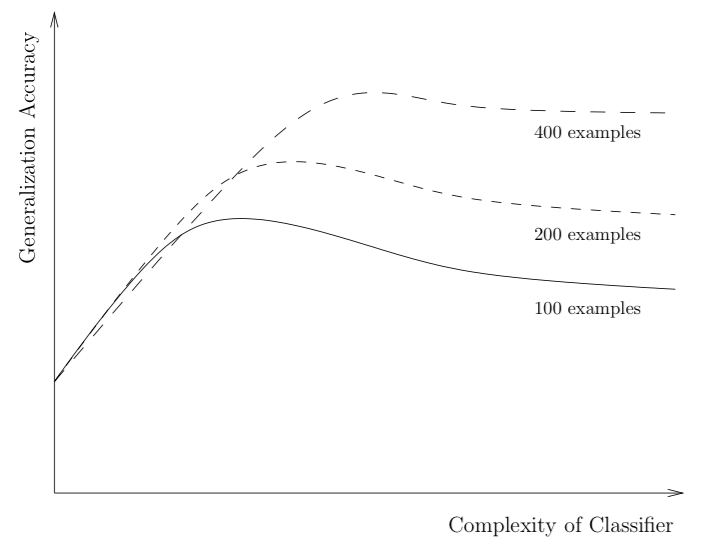
\includegraphics[width=0.8\textwidth]{img/3tradeoff}
  \caption[Tradeoff in empirical learning ]{Tradeoff in empirical learning from \cite{dietterich2003}. The
generalization accuracy is not affected by the amount of examples for low
complex classifiers. However, for some more complex classifiers, the number of
examples improves the generalization accuracy. The key is to find the best
generalization accuracy and the lowest complex classifier with the available
training data. }
  \label{fig:tradeoff}
\end{figure}

\subsection{The bias-variance tradeoff} \label{sec:biasvar}

A very complex models will fit the training data better (low bias) but it could
overfit it and generalise poorly (high variance), this is also called the
bias-variance tradeoff.  

Figure \ref{fig:traintesterror} shows {\em prediction or estimation error} for
training and testing sample.  In general, in the training sample prediction
error is decreasing with more complex models but it overfit the data and it is
not a good model for the test data. 

\begin{figure}[!h]
  \centering
  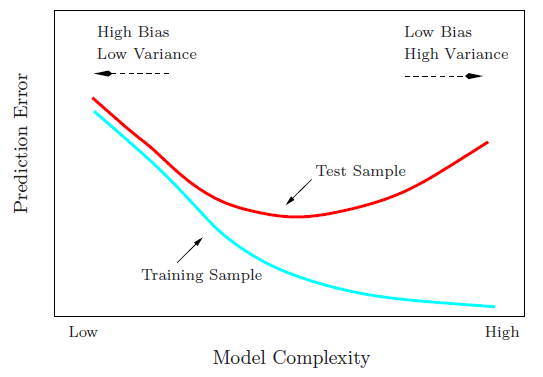
\includegraphics[width=0.8\textwidth]{img/model_complexity}
  \caption[Training and test error]{Training and test error. Image source is
\cite{friedman2001elements}.The blue curve represents the training error which
decreases with more complex models. However, the model starts to overfit the
data reducing the generalisation capacity of the model,this occurs when the
prediction error in the test sample starts to increase (red curve).}
  \label{fig:traintesterror}
\end{figure}

Models learning error can be split into two main components: error due to bias
and error due to variance. Bias measures the prediction error of the model
$\hat{f}$ from the real value, see equation~\eqref{eq:biastrade}. Variance is
taken as the variability of a model prediction for a given data point or its
sensitivity to small fluctuations in the input data, see equation
\ref{eq:variancetrade}.

If we have a learning model $\hat{f}$, its expected generalisation error on a
testing sample $x$ can be decomposed as shown in equation~\eqref{eq:bvtrade} (proof
in \cite{geman1992neural}):

\begin{align}
\label{eq:bvtrade}
\mathrm{E}\Big[\big(y - \hat{f}(\mathbf{x})\big)^2\Big]
 & = \mathrm{Bias}(\hat{f}(\mathbf{x}))^2 + \mathrm{Var}(\hat{f}(\mathbf{x})) + \sigma^2
\end{align}
\noindent where:
\begin{align}
 \mathrm{Bias}(\hat{f}(\mathbf{x})) &= \mathrm{E}\big[\hat{f}(\mathbf{x})\big] - f(\mathbf{x}) \label{eq:biastrade}\\
 \mathrm{Var}(\hat{f}(\mathbf{x})) &= \mathrm{E}\Big[ \big( \hat{f}(\mathbf{x}) - \mathrm{E}[\hat{f}(\mathbf{x})] \big)^2 \Big]  \label{eq:variancetrade}
\end{align}


Figure \ref{fig:bvtradeoff} shows how
testing error can be decomposed into bias and variance components. 
The bias shown in equation~\eqref{eq:biastrade} can be obtain through resampling
of the input data $x$, therefore an average of the predicted values can be
calculated. If these prediction values are substantially different to the true
value, the bias will be high.

\begin{figure}[!h]
  \centering
  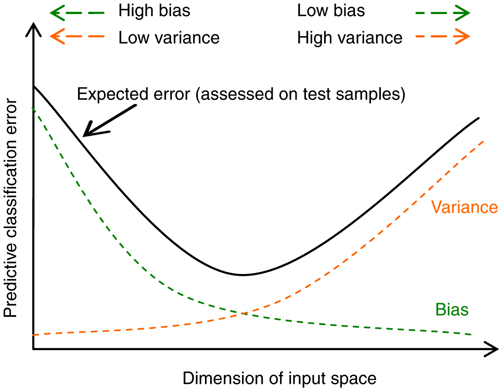
\includegraphics[width=0.8\textwidth]{img/biasvariancetradeoff}
  \caption{Bias variance tradeoff}
  \label{fig:bvtradeoff}
\end{figure}

The error due to variance is the amount by which the prediction, over one
training set, differs from the expected predicted value, over all the training
sets. Variance measures how inconsistent are the predictions from one another,
over different training sets, not whether they are accurate or not
\cite{gutierrez2015machine}.

\subsection{Generalised Cross Validation}
This bias-variance tradeoff is the reason why the 
data is usually divided in three subsets: training, validation and
testing set. The training set is used to construct the model, the validation set
to estimate the generalisation error and finally the testing set to estimate
the accuracy of the model. Usually the partition is 50\% for training, 25\%
for validation and 25\% for testing purposes. When the
amount of data is limited, this procedure can be extended to
a Cross Validation (CV) approach \cite{geisser1975} . Various splitting strategies lead to various CV
estimates. In K-fold cross-validation  \cite{stone1974} the training data is divided randomly into
K distinct subsets, then the model is trained using K-1 subsets, and tested on
the remaining subset. The process of training and testing is then repeated for
each of the K possible choices of the subset omitted from the training. The
average performance on the K omitted subsets is the estimate of the
generalisation performance.

%Another way to control the complexity of the model is to include in the
%optimisation function not only the generalisation error but a penalisation of
%high complex models. 


%Since we don't know the data we want to predict, the bias-variance tradeoff is not directly useful to determine $\lambda$. Many techniques have been developed to determine a suitable value for the regularization parameter. However, when no information is available on the error, one of the most popular techniques is the Generalized Cross Validation (GCV) \cite{bauer2011}. GCV originates from the older method leave-one-out Cross Validation.

%The leave-one-out cross validation method determine a regularization parameter that minimises the average of the squared predictions errors using each solution to predict the missing data value.

%'---------------------------http://robjhyndman.com/hyndsight/crossvalidation/
%When the data are not independent cross-validation becomes more difficult as leaving out an observation does not remove all the associated information due to the correlations with other observations. 

%For time series forecasting, a cross-validation statistic is obtained as
%follows: fit the model to the data $y1,\dots,yt$ and let $y^t+1$ denote the forecast
%of the next observation. Then compute the error $et+1=yt+1-y^t+1$ for the
%forecast observation.  Repeat step 1 for $t=m,\dots,n−1$ where m is the minimum number
%of observations needed for fitting the model.
%Compute the MSE from $em+1∗,…,en∗$.

%An excellent and comprehensive recent survey of cross-validation results is Arlot and Celisse (2010)

%---------------------------------------------------

\subsection{Regularization}\label{sec:regularization}

Regularization can be understood using two contexts: learning theory
(probabilistic) and inverse problems (deterministic). In the context of
learning, regularization refers to techniques allowing to avoid over-fitting and
the desire property of the selected estimator is to perform well on new data (to
generalise), e.g. regularized least squares. In the context of inverse problems,
regularization objective is to stabilise, with respect to noise, a possibly
ill-conditioned matrix inversion problem e.g spectral cut-off and Tikhonov
regularization or ridge regression (RR) \cite{ tikhonov1977}. More details in section \ref{app:effcomp}.

In particular, it is well known that regularization schemes such as RR or
Tikhonov regularization can be effectively used in the context of learning
\cite{vito2005}.

Tikhonov introduced a regularization which ensures well-posedness and
generalisation of ERM, i.e prevents overfit, by constraining the hypothesis
space $\mathscr{H}$ usually called regularised ERM or Tikhonov regularisation.

%Tikhonov regularisation minimised over the hypothesis space $\mathscr{H}$ for a
%fixed positive parameter $\lambda$ the following:
Tikhonov regularisation considers a functional of the form:

\begin{equation} 
\label{eq:rerm}
R_{\text{emp}}[f] = \frac{1}{n} \sum_{i=1}^n V(f(x_i),y_i) + \lambda \mathcal{R}(f)
\end{equation}

\noindent where $X \subseteq \mathbb{R}^m$ and $Y = \mathbb{R}$ , $V$ is the
loss function defined in the equation~\eqref{eq:lossfunction} and $\mathcal{R}(f)$
is the regulariser, a penalisation on $f$. One example of regularisation in
linear models is Ridge Regression (RR), which is a regularised least squares
method.

\subsection{Ridge Regression}

Ridge regression (RR) was independently proposed by Tikhonov \cite{tikhonov1963}
and Phillips \cite{phillips1962}. 

RR corresponds to a regularised least squares
method. The least squares (LS) method is a well known way to solve a regression
problem.  

LS method consists of minimising the sum of squared errors:
\begin{eqnarray*}
\label{eq:lsm}
 J(\mathbf{X}) =& \displaystyle \sum_{t=1}^n (f(\mathbf{x}_t)-y_t)^2 \\
 =&\displaystyle \sum_{t=1}^n (\mathbf{\mathbf{A}}^\top {\mathbf{x}}_t-y_t)^2 \\
 =& \| \mathbf{A}\mathbf{\mathbf{X}} - \mathbf{Y} \|_2^2 
\end{eqnarray*}

\noindent where 
\begin{equation}
\label{eq:RRdefinitions}
\mathbf{X} = 
\left[
  \begin{array}{cccc}
    \vertbar & \vertbar &        & \vertbar \\
    \mathbf{x}_{1}    & \mathbf{x}_{2}    & \ldots & \mathbf{x}_{n}    \\
    \vertbar & \vertbar &        & \vertbar 
  \end{array}
\right]
\quad , \quad
\mathbf{A} = 
\left[
  \begin{tabular}{c>{$}c<{$}c}
    --- & \mathbf{a}^{\top}_{1} & ---\\
    --- & \mathbf{a}^{\top}_{2} & ---\\
    & \vdots & \\
    --- & \mathbf{a}^{\top}_{m} & ---
  \end{tabular}
\right]
\quad \text{and} \quad
\mathbf{Y} = 
\left[
  \begin{array}{cccc}
    \vertbar & \vertbar &        & \vertbar \\
    \mathbf{y}_{1}    & \mathbf{y}_{2}    & \ldots & \mathbf{y}_{n}    \\
    \vertbar & \vertbar &        & \vertbar 
  \end{array}
\right]
\end{equation}

\noindent and $f(\mathbf{x}_t)={\mathbf{A}}^\top {\mathbf{x}}_t$. 

To solve equation~\eqref{eq:lsm} is equivalent to find a solution of:
\begin{equation}
\label{eq:regproblem}
\underset{m \times n}{\mathbf{A}} \enskip \underset{n \times
l}{\mathbf{\mathbf{X}}} = \underset{m \times l}{\mathbf{Y}} \;.
\end{equation}

The optimal solution for $\mathbf{\mathbf{X}}$ is:
\begin{equation}
\label{eq:MP}
\mathbf{\mathbf{X}}= \mathbf{A}^+ \mathbf{Y} \;,
\end{equation}

\noindent where $\mathbf{A}^+$ is the Moore-Penrose pseudo-inverse
which can be written as follows: 

\begin{equation}
\label{eq:pseudoinverse}
\mathbf{A}^+= (\mathbf{A}^\top \mathbf{A})^{-1}\mathbf{A}^\top \, .
\end{equation}





However, when $\mathbf{A}$ is not full rank, i.e
$rank(\mathbf{A})=k <  n \leq m$, $\mathbf{A}^\top \mathbf{A}$ is
always singular and equation~(\ref{eq:pseudoinverse}) cannot be used.
More generally, the pseudo-inverse is best computed using the compact
singular value decomposition (SVD) of $\mathbf{A}$:

\begin{equation}
    \label{eq:compactsvd}
    \underset{m \times n}{\mathbf{A}}=
    \underset{m \times k}{\mathbf{U_1}} \enskip
    \underset{k \times k}{\mathbf{\Sigma_1}} \enskip
    \underset{k \times n}{\mathbf{V_1}^\top} \;,
\end{equation}

\noindent as follows

\begin{equation}
\label{eq:pseudoinversesvd}
\mathbf{A}^+ = \mathbf{V_1\Sigma_1^{-1}U_1^\top} \;.
\end{equation}

Proof can be found in the appendix section \ref{app:pseudoproof}.


In order to avoid the singularity of the matrix $\mathbf{A}^\top \mathbf{A}$, a regularisation term $\lambda$ is introduced: 

\begin{equation}
\label{eq:RRproblem} 
J(\mathbf{\mathbf{X}}) =  \| \mathbf{A}\mathbf{\mathbf{X}} - \mathbf{Y} \|_2^2  + \lambda
 \| \mathbf{\mathbf{X}}\| ^2 \;,
\end{equation}

\noindent which optimal solution $\mathbf{\mathbf{X}}_*$ is well known: 

\begin{equation}
\label{eq:optsolRR}
\mathbf{\mathbf{X}}_*=(\mathbf{A}^\top \mathbf{A}+\lambda \mathbb{I})^{-1}\mathbf{A}^\top y \;.
\end{equation}

Proof can be found in section \ref{app:rroptsection}.



The method is called ridge regression because the term $\lambda \mathbb{I}$ adds positive entries along the diagonal (ridge) to avoid the
singularity of the covariance matrix $\mathbf{A}^\top \mathbf{A}$. This addition ensures that all of the covariance matrix eigenvalues will be strictly greater than 0, i.e the solution becomes unique.

\subsection{The Lambda parameter}

The additional term $\lambda \|\mathbf{\mathbf{X}}\|_2^2$ in the optimisation
problem shown in equation~(\ref{eq:RRproblem}) has two effects on the solution:
shrinks the coefficients towards zero and improves the conditioning of the
problem.

When $\mathbf{A}$ is orthonormal then $\mathbf{A}^\top \mathbf{A} =\mathbb{I}$ and there is a simple relation between the ridge estimator and the OLS estimator:
\begin{eqnarray*}
\mathbf{X}_* (\lambda) &=& (\mathbf{A}^\top \mathbf{A}+\lambda \mathbb{I})^{-1}\mathbf{A}^\top \mathbf{Y} \\
 &=& (\mathbb{I} + \lambda \mathbb{I})^{-1} \mathbf{A}^\top \mathbf{Y} \\
 &=&(1+\lambda)^{-1} \mathbb{I} \mathbf{A}^\top \mathbf{Y} \\
 &=&(1+\lambda)^{-1} (\mathbf{A}^\top \mathbf{A})^{-1}\mathbf{A}^\top \mathbf{Y} \\
 &=&(1+\lambda)^{-1} \mathbf{X}
\end{eqnarray*}

Figure~\ref{fig:shrinks} shows a visual example of the shrinking of the
coefficients:

\begin{figure}[h!]
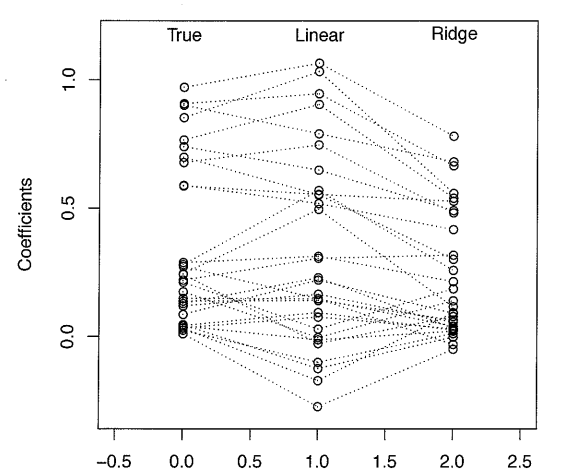
\includegraphics[width=0.5\linewidth]{img/shrinks}
\caption{Shrink of regression coefficients}
\label{fig:shrinks}
\end{figure}


On the other hand, the effect of adding the term $\lambda \mathbb{I}$
to the matrix $\mathbf{A}^\top \mathbf{A}$
(equation~(\ref{eq:optsolRR})) improves its condition number since it
increases its diagonal values when $\lambda > 0 $.  The matrix
$\mathbf{A}^\top \mathbf{A}$ is symmetrical ($(\mathbf{A}^\top
\mathbf{A})^\top = \mathbf{A}^\top \mathbf{A}$) and therefore
diagonalizable.  If we know the eigenvalue decomposition of $\mathbf{A}
= \mathbf{U\Sigma V^\top}$, then:

\begin{eqnarray*}
\mathbf{A}^\top \mathbf{A}+\lambda \mathbb{I}&=&\mathbf{V\Sigma^2
V}^\top + \lambda \mathbf{V} \mathbf{V}^\top\\ &=&\mathbf{V}
(\mathbf{\Sigma}^2+\lambda\mathbb{I}) \mathbf{V}^\top \, ,
\end{eqnarray*}

\noindent where

\begin{equation*}
\mathbf{\Sigma}^2+\lambda\mathbb{I}=
\begin{bmatrix}
\sigma^2_1 + \lambda & \, & \, \\
\, & \sigma^2_2 +\lambda & \, \\
\, & \, & \ddots & \, \\
\, & \, & \, & \sigma^2_n +\lambda \, .
\end{bmatrix}
\end{equation*}

\noindent where $\sigma_1 \geq \sigma_2 \geq \dots \geq \sigma_n$.

Since the condition number of a matrix $\mathbf{A}$ is defined as:

\begin{equation*}
	\kappa = \|\mathbf{A}\| \|\mathbf{A}^{-1}\|
\end{equation*}

If matrix $\mathbf{A}$ is non-singular, its condition number can be
expressed in terms of its singular values. The effect of adding the
regularization term affects the condition number as follows:
\begin{eqnarray*}
\kappa_{ols} &=& \|\mathbf{A}\| \|\mathbf{A}^{-1}\|=\frac{\sigma_1}{\sigma_n} \\
\kappa_{ridge} &=& \|\mathbf{A}^\intercal \mathbf{A} + \lambda \mathbb{I}\| 
\|(\mathbf{A}^\intercal \mathbf{A} + \lambda \mathbb{I})^{-1}\|=\frac{\sigma_1+\lambda}{\sigma_n + \lambda} \;.
\end{eqnarray*}

It is easy to see that the term $\lambda$ improves the condition number: 

\begin{equation*}
        \frac{\sigma_1+\lambda}{\sigma_n + \lambda} <
        \frac{\sigma_1}{\sigma_n} \,  \qquad \forall \quad \lambda > 0
\end{equation*}


However, $\lambda$ cannot be too large. Tipically $\lambda$ is small and its
magnitude depends on the matrix $\mathbf{A}$.

For rank deficient matrices we know that $\text{det}(\mathbf{A A^\top})=0$, adding the
term $\lambda \mathbb{I}$ we have that $\text{det}(\mathbf{A A^\top}+\lambda \mathbb{I}) =
p(\lambda)$ where $p(\lambda)$ is a polynomial of degree $n$ ($\mathbf{A}$ is
$m \times n$). The zeros of $p(\lambda)$ are discretes, so it can be represented
as:

\[
p(\lambda) =
\lambda(\lambda-\lambda_1)^{n_1}(\lambda-\lambda_2)^{n_2}\dots(\lambda-\lambda_s)^{n_s}
\]

\noindent where $n_1 + n_2 + \dots + n_s = n$.

This means that $\lambda$ must be small in order to ensure that $p(\lambda)$
does not vanish.


\subsection{Selection of Lambda}

One of the ways to determine parameter $\lambda$ is using the bias-variance tradeoff (see section~\ref{sec:biasvar}). This parameter is crucial for ridge regression since it could
reduce the expected prediction error by reducing variance, considering a biased
estimator. 
It is known that the prediction error can be express as a decomposition between bias and variance.

The solution of OLS is well known $\hat{\mathbf{X}}=(\mathbf{A}^\top \mathbf{A})^{-1}\mathbf{A}^\top \mathbf{Y}$, and its bias ($Bias(\hat{f}(\hat{\mathbf{X}})$)  is 0 (Proof in section \ref{app:biasandvariance}).

The bias of ridge regression when $\mathbf{A A^\top}$ is non-singular
can be obtained expressing ridge regression solution
$\mathbf{\lambda}$ in terms of OLS solution $\hat{\mathbf{X}}$:

\begin{equation}
 Bias(\mathbf{X}(\lambda))  = \mathbf{W} \mathbf{X} - \mathbf{X} \neq 0 
 \end{equation}
 
 \noindent where $\mathbf{W}  = (\mathbb{I} + \lambda (\mathbf{A}^\top
\mathbf{A})^{-1})^{-1}  $


The variance of OLS is:

\begin{equation*}
Var(\hat{\mathbf{X}}) = \sigma^2 (\mathbf{A}^\top \mathbf{A} )^{-1}
\end{equation*}

\noindent and the variance of ridge regression is:

\begin{equation*}
Var(\mathbf{X}(\lambda)) = \sigma^2 \mathbf{W}(\mathbf{A}^\top \mathbf{A} )^{-1}\mathbf{W}^\top
\end{equation*}

Proof in section \ref{app:biasandvariance}.

\begin{figure}[h!]
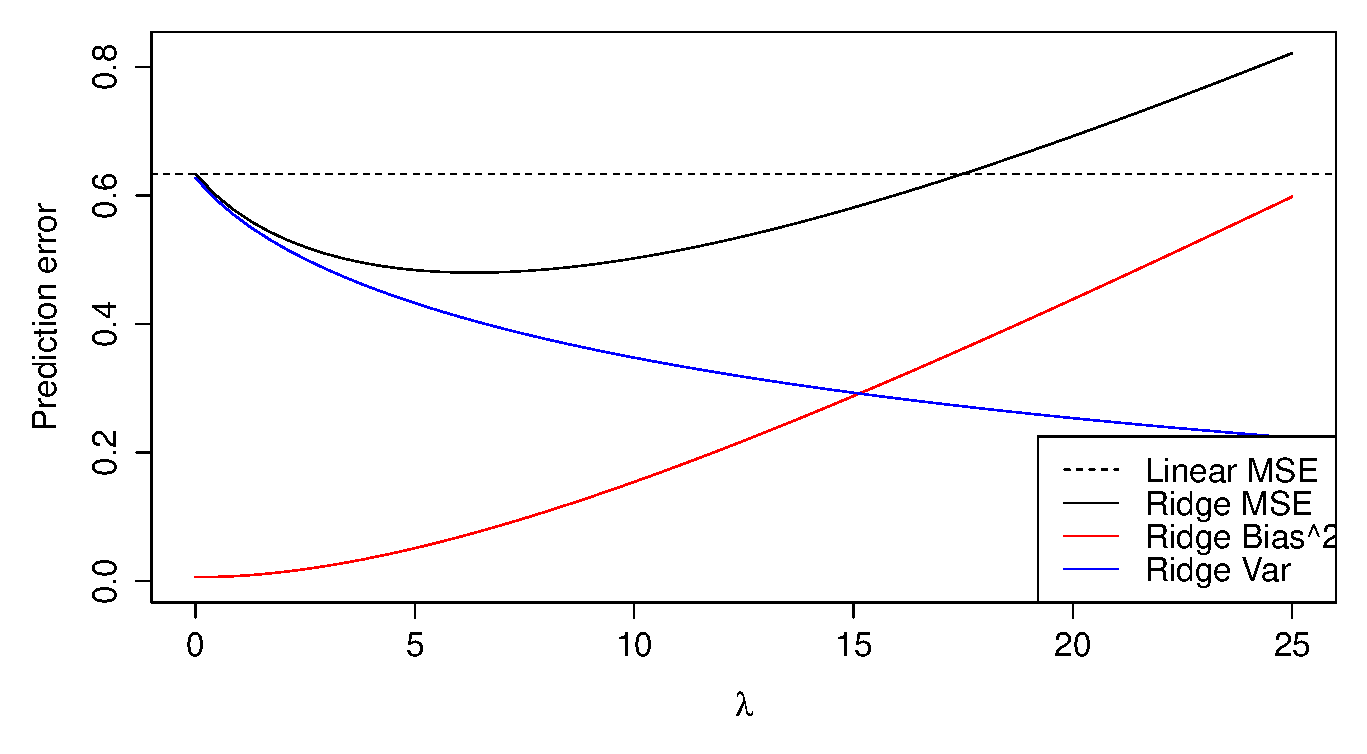
\includegraphics[width=\linewidth]{img/biasvariance}
\caption[Bias-variance tradeoff depending on lambda]{Bias-variance tradeoff depending on lambda. Dotted line corresponds to OLS prediction error (invariant with lambda). Black line corresponds to RR prediction error which can be decomposed in $Bias^2$ (in red) + Variance (in blue).}
\label{fig:biasvariance}
\end{figure}	


The figure~\ref{fig:biasvariance} shows the bias-variance tradeoff
given by equation~(\ref{eq:bvtrade}). 

Despite OLS has zero bias,
its variance is greater than ridge for small values of $\lambda$.
It can be shown that, in terms of prediction error, ridge (black line)
is lower than OLS (dotted line)~\cite{hoerl1970}. Ridge regression shows an
increasing squared bias and a decreasing variance. See proof in section \ref{app:rrbiasvar}.



\subsection{Machine learning algorithms}
In recent years many successful machine learning applications have been developed. Artificial neural networks (ANN) and Support Vector Machines (SVM) have been some of the most popularly used machine learning algorithm \cite{haykin1998}. Historically, SVMs emerged after ANN.

The main characteristics of neural networks are that they have the ability to learn
complex nonlinear input-output relationships, they use sequential training procedures 
they adapt themselves to the data.

ANN is inspired by biological learning systems organised into layers and have unidirectional connections between the layers, feed-forward networks  (FFN) are the most used.  FFN consist of a series of layers. The first layer has a connection from the network input. Each subsequent layer has a connection from the previous layer. The final layer produces the network's output. Figure \ref{fig:ffn} shows a FFN with its different layers.

\begin{figure}[!h]
  \centering
  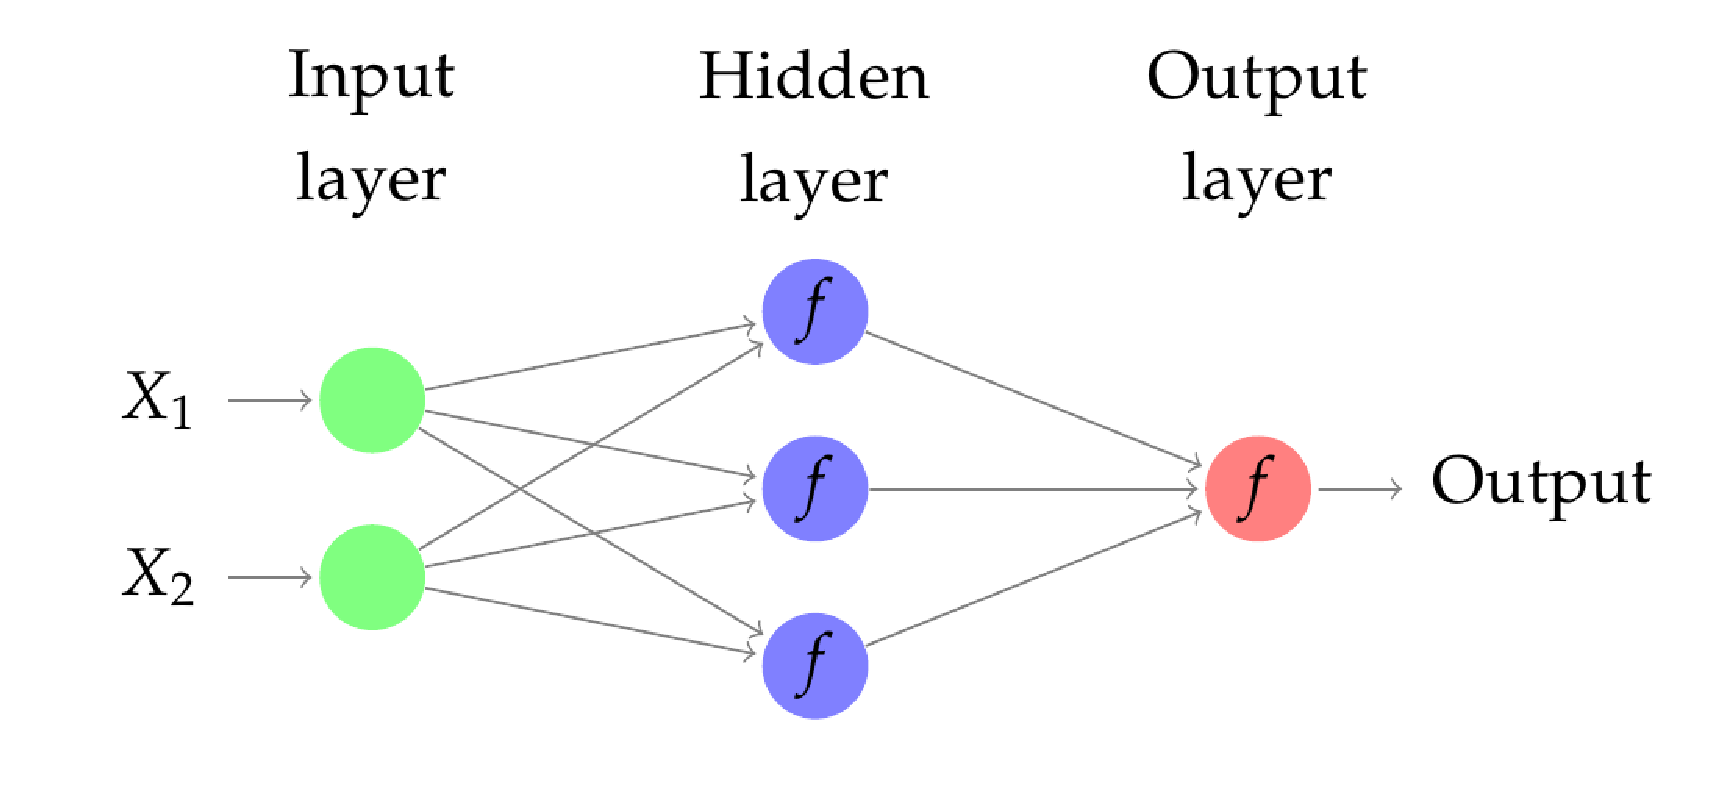
\includegraphics[width=0.8\textwidth]{img/ffn}
  \caption[Feed-forward neural network (FFN)]{Feed-forward neural network (FFN). FNN consists of an input layer, an output layer and at least one hidden layer between the input and output layer. }
  \label{fig:ffn}
\end{figure}


Support Vector Machine (SVM) was introduced in 1992 by Vapnik and his coworkers
\cite{boser1992}. In its original form, SVM is a training algorithm for linear classification. Only later it was used for regression, principal component analysis, novelty detection and also for non-linear case.  However, unlike ANN, it is very well 
based on theory in statistical learning \cite{cortes1995}.  SVM tunes the capacity of 
maximising the margin between the training patterns and the decision boundary. The
solution is expressed as a linear combination of supporting patterns, which are the training patterns close to the decision boundary, called the support vectors.

The major difference between SVM and ANN is the error optimisation. In ANN, the aim of learning is to obtain a set of weight values which minimise the training error while training adjust the capacity of the machine.

For nonlinear case, SVM mapped the data sets of input space into a higher dimensional feature space, which is linear and the large margin learning algorithm is then applied. However, the mapping can be implicitly done by kernel functions. In the high dimensional feature space, simpler and linear hyper plane classifiers that have maximal margin between the classes can be obtained.

%\subsection{Kernel methods}
%Kernel functions may be used to introduce a nonlinear separation
%in input space despite the linear classifier in decision space
\newpage
\section{Online learning} \label{sec:onoffline}

Online learning is a supervised machine learning framework that is useful when
we have sequential access to a sample only once.  This differs from the
classical batch learning, where there is an entire data set available and the
learner can build the internal model without any limits in accessing the data.
In batch learning, there is time enough to carefully analyse the dataset, build
large predictive models and combine them in a sophisticated way. However, when
execution time is critical and new data is required to be included in the model,
online learning algorithms are a better option.

In batch learning, the training phase is commonly a computationally expensive
process. Therefore, when new data arrives it can't be included easily into the
model. Moreover, it could happen that we won't have enough time to process the
new data before more data arrives. In online learning algorithms there is no
training phase, the model is updated and evaluated at every time step. This
model updating is computationally less expensive than a training phase.

Online algorithms allow incremental learning by processing one instance at a
time. This is done updating the current model instead of building the model from
scratch.

Online learning is also useful when some past data may be irrelevant
or we want to improve computational efficiency. However, the use of less
historical data could affect accuracy.

The goal of online learning is the same as batch learning, predicting targets as
accurate as possible. For example, stock market prediction can be seen as online
learning. The algorithm makes a prediction of the stock, little time after the
real stock price is available, this information can be incorporated to the
learner to further improve the prediction accuracy. In general, there is too
much data available in an online learning setup, the data set grows
continuously. Offline learning has equal or superior accuracy compared to online
learning when the same amount of data is used.

Classic statistical theory of sequential prediction enforces strong assumptions
on the statistical properties of the input sequence (for example, stationary
stochastic process). However, these assumptions can be unknown or change over
time. In online learning there is no previous assumption about the data and the
sequence is allowed to be deterministic, stochastic or even adaptive.  

Moreover, in case we receive data streams, ANN or SVM cannot introduce new
information into the model without a re-training process, so we will have to use
the same non-updated model until we decide to compute another one if it is
possible.  Online learning algorithms allow one example at a time to be
introduced into an existing model incrementally \cite{vovk2005}. This is
extremely important when the problem has large data streams and real-time
forecasting must be done.  This is the most common scenario when we want to
forecast a wide range of data such as stock prices and volatilities, electricity
power, intrusion detection, web-mining, server load, etc.  Besides, many
problems of high interest in machine learning can be treated as online ones and
they can also use these types of algorithms.

The online learning framework was first introduced in the perceptron algorithm
\cite{rosenblatt58}. There are several other widely used online methods such as
passive-aggressive \cite{crammerETall2006}, stochastic gradient descent
\cite{zhang2004}, aggregating algorithm \cite{vovk2001} and the second order
perceptron \cite{cesa-bianchi2005}.  In \cite{cesa-bianchi2006} an in-depth
analysis of online learning is provided. Applications in finance has been widely used: study presented by~\cite{arce+salinas2012} applied ridge regression in an online context and more recently, time series forecasting using online learning has been presented~\cite{anavaetAl2013}.

The motivation for online learning is to obtain computational efficiency and
tackle the shifting problem, i.e. that the distribution of the data is unknown
or changes over time. Online learning algorithms can deal with this problem
because they have a tracking ability which is a strategy based on retaining weak
dependence on past examples by using two types of models: 

\textit{a)} \textbf{memory boundedness:} consists of limiting the number of
support vectors in order to improve computational efficiency. One example of
this is the budget perceptron~\cite{crammeretal2004} which reduces the number of
examples used for prediction. Alternatively, in the forgetron
algorithm~\cite{dekeletal2008} the damage caused by removing old examples is
discussed, which can be avoided by removing samples with small influences. Other
examples are the sliding window kernel (RLS)~\cite{vanvaerenberghetal2006},
which only considers a sliding window of the most recent data, and in
\cite{arce+salinas2012} is shown a variant of aggregating algorithm for
regression~\cite{vovk2001} considering only a sliding window of the most recent
data, optimising also common matrix operations.

\textit{b)} \textbf{weight decay:} one example of this is the shifting
perceptron algorithm which implements an exponential decaying scheme for the
examples~\cite{cavallantietal2007}.  Performance of an online learning algorithm
is measured by the cumulative loss it suffers along its run on a sequence of
examples. In order to minimise this loss, the learner may update the hypothesis
after each round so as to be more accurate in later rounds.


There is sometimes confusion about online and incremental learning concepts.
Incremental learning refers to any online learning process that learns the same
model as would be learnt by a batch learning algorithm. 

Incremental learning is useful when the input to a learning process is stream
data, with the need or desire to be able to use the result of learning at any
point in time, based on the input observations received so far. 

Incremental learning is very useful when there is no need to record fundamental
data and only a summary needs to be retained. Due to this, incremental
algorithms are often characterised as memoryless, because no memory of past data
is required.  The algorithm is online but not incremental if it doesn't produce
the same result for all observations that the corresponding batch algorithm
would for these same observations.
\newpage
Algorithm~\ref{alg:onlinealg} shows the online learning algorithm structure:
\begin{algorithm}[ht]
\begin{algorithmic}[1]
    \STATE Receives input $\mathbf{x}_t$
    \STATE Makes prediction $\mathbf{\hat{y}}_t$
    \STATE Receives response $\mathbf{y}_t$
    \STATE Incurs loss $l_t(\mathbf{y}_t,\mathbf{\hat{y}}_t)$
\end{algorithmic}
\caption{Structure of a Learning System}
\label{alg:onlinealg}
\end{algorithm}
\noindent where $l$ is some loss function. Performance is later measured after
$T$ trials as:
\begin{equation*}
L_T = \sum_{t=1}^T l_t(\mathbf{y}_t,\mathbf{\hat{y}}_t)
\end{equation*}
The objective is to minimise this loss function for all instances.
The quality of online learning algorithms is measured by a quantity known as
regret which is the difference between the performance of the online algorithm
and its optimal predictor $E^* \in \Theta$ given by:

\begin{equation*}
L^*_T= \text{min}_{E \in \Theta} L_T^E \, ,
\end{equation*}


\noindent where $L_T^E = \sum_{t=1}^T
l_t(\mathbf{y}_t,\mathbf{y}^E_t)$ and $\mathbf{y}^E_t$ is the expert estimation. 

Therefore regret is defined as:

\begin{equation*}
R_T = L_T - L^*_T
\end{equation*}

\subsection{Online Ridge Regression}

Online RR is the online formulation of the regularised Least Squares method
and is based on the following equivalent formulation of the RR optimal solution.

Since 
\begin{equation}
\label{eq:notation}
	\mathbf{A} = 
\left[
  \begin{tabular}{c>{$}c<{$}c}
    --- & \mathbf{a}^{\top}_{1} & ---\\
    --- & \mathbf{a}^{\top}_{2} & ---\\
    & \vdots & \\
    --- & \mathbf{a}^{\top}_{m} & ---
  \end{tabular}
\right]
\quad \text{and} \quad
\mathbf{B} =
\left[
  \begin{tabular}{c>{$}c<{$}c}
    --- & \mathbf{b}_{1} & ---\\
    --- & \mathbf{b}_{2} & ---\\
    & \vdots & \\
    --- & \mathbf{b}_{m} & ---
  \end{tabular}
\right]
\end{equation}

\noindent equation~(\ref{eq:optsolRR}) can also be written as: 

\begin{eqnarray*}
\label{eq:RReapand}
\mathbf{\mathbf{X}}_{\text{ridge}}&=&(\mathbf{A}^\top \mathbf{A}+ \lambda
\mathbb{I})^{-1}\mathbf{A}^\top \mathbf{Y} \\
&=& \displaystyle \big (\sum_{t=1}^m
\mathbf{a}_t \mathbf{a}_t  ^\top + \lambda \mathbb{I}\big )^{-1}
\sum_{t=1}^m \mathbf{a}_t \mathbf{y}_t \, .
\end{eqnarray*}

Lets define $\displaystyle\mathbf{S}= \sum_{t=1}^m \mathbf{a}_t
\mathbf{a}_t  ^\top + \lambda \mathbb{I} $ and $\mathbf{W}=
\displaystyle\sum_{t=1}^m \mathbf{a}_t \mathbf{y}_t$, so the
algorithm~\ref{alg:RR} shows the iterative formulation:

\begin{algorithm}[H]
\begin{algorithmic}[1]
\REQUIRE $\,$ \\
$\{\mathbf{a}_1,\dots,\mathbf{a}_{m} \}$: $m$ input vectors \\
$\{\mathbf{y}_1,\dots,\mathbf{y}_{m} \}$: $m$ target vectors \\
$\lambda$: regularization parameter \\
\ENSURE  $\,$ \\
$\{f(\mathbf{a}_1),\dots,f(\mathbf{a}_{m}) \}$: model predictions \\
\STATE Initialize $\mathbf{S}=\lambda \mathbb{I}$
and $\mathbf{W}=0$
\FOR { $t = 1$ to $m$ }
	\STATE read new $\mathbf{a}_t$
	\STATE $\mathbf{X}=\mathbf{S}^{-1}\mathbf{W}$
	\STATE output prediction $f(\mathbf{a}_t) = \mathbf{X}^\top \mathbf{a}_t$
   	\STATE $\mathbf{S} = \mathbf{S} + \mathbf{a}_t \mathbf{a}_t^\top$
   	\STATE Read new $y_t$
    	\STATE $\mathbf{W} = \mathbf{W} + \mathbf{a}_t \mathbf{y}_t$
\ENDFOR
\end{algorithmic}
\caption{Online Ridge Regression}
\label{alg:RR}
\end{algorithm}



\subsection{The Aggregating Algorithm for Regression}

The AAR, proposed by Vovk~\cite{vovk2001} (also known as Vovk-Azoury-Warmuth predictor ~\cite{azoury2001}), is an application of the aggregating
algorithm to the problem of regression. The idea is introduce the new input
vector $\mathbf{x}_{m+1}$ to solve the model parameters: 

\begin{equation}
\label{eq:AARexpand}
\mathbf{X}_{aar} = \displaystyle \left(\sum_{t=1}^{m+1}
\mathbf{a}_t \mathbf{a}_t  ^\intercal + \gamma \mathbb{I} \right) ^{-1}
\sum_{t=1}^m \mathbf{a}_t \mathbf{y}_t \, .
\end{equation}

\begin{algorithm}[ht]
\begin{algorithmic}[1]
\REQUIRE $\,$ \\
$\{\mathbf{a}_1,\dots,\mathbf{a}_{m} \}$: $m$ input vectors \\
$\{\mathbf{y}_1,\dots,\mathbf{y}_{m} \}$: $m$ target vectors \\
$\lambda$: regularisation parameter \\
\ENSURE  $\,$ \\
$\{f(\mathbf{a}_1),\dots,f(\mathbf{a}_{m}) \}$: model predictions \\
\STATE Initialize $\mathbf{S}=\lambda \mathbb{I}$
and $\mathbf{W}=0$
\FOR { $t = 1$ to $m$ }
	\STATE read new $\mathbf{a}_t$
   	\STATE $\mathbf{S} = \mathbf{S} + \mathbf{a}_t \mathbf{a}_t^\intercal$
	\STATE $\mathbf{X}=\mathbf{S}^{-1}\mathbf{W}$
	\STATE output prediction $f(\mathbf{a}_t) = \mathbf{X}^\intercal \mathbf{a}_t$
   	\STATE Read new $\mathbf{y}_t$
    	\STATE $\mathbf{W} = \mathbf{W} + \mathbf{a}_t \mathbf{y}_t$
\ENDFOR
\end{algorithmic}
\caption{{\em The aggregating algorithm for regression}}
\label{alg:AAR}
\end{algorithm}

If we define $\displaystyle\mathbf{S}= \sum_{t=1}^{m+1} \mathbf{a}_t
\mathbf{a}_t  ^\intercal + \gamma \mathbb{I} $ and $\mathbf{W}=
\displaystyle\sum_{t=1}^m \mathbf{a}_t \mathbf{y}_t$, the
algorithm~\ref{alg:AAR} is slightly different to the algorithm~\ref{alg:RR}, 
which updated matrix $\mathbf{S}$ before making the prediction.

\subsection{Competitive analysis}

Competitive analysis was designed for analysing the performance of an online algorithm compared with its optimal offline algorithm. An optimal offline algorithm can view the sequences of requests in advance. The effectiveness of an online algorithm \cite{sleator1985} may be measured by its competitive ratio which is the worst-case ratio of the online algorithm and the optimal offline algorithm.




%Despite the bias-variance tradeoff provides a conceptual framework for
%determining a good model, is not directly useful. Some popular methods
%for determine model selection are:
%
%\begin{itemize}
%    \item Akaike information criterion (AIC) (Akaike, 1974)
%    \item Bootstrap-based selection (Efron and Tibshirani, 1997)
%    \item Cross-validation (Stone, 1974)
%\end{itemize}
%
%On the other hand, $\lambda$ can also be used to reduce computational time as it
%is shown in equation~(\ref{eq:taylor}). Golub (~\cite{golub1965}) suggested that
%$\lambda$ be chosen so that:
%
%\[
%\frac{\lambda}{\lambda + \delta^2} < 0.1
%\]
%
%\noindent where $\delta$ is a lower bound of the smallest non-zero singular
%value $\sigma_k$. One approach is to choose the greatest lower bound for
%$\delta=\sigma_k$. Hence:
%
%\[
%\frac{\lambda}{\lambda + \sigma_k^2} < 0.1
%\]
%
%\noindent if we choose $\lambda=\beta \sigma_k^2$ then we get the following
%relation:
%
%
%\[
%\frac{\beta \sigma_k^2}{\beta \sigma_k^2 + \sigma_k^2} =
%\frac{\beta}{\beta+1} < 0.1 \Rightarrow \beta < \frac{1}{9}  
%\]
%
%Experiments done by ~\cite{coleman+sun2010} have shown that $\beta = 0.01$
%produces satisfactory results. This means that $\lambda = 0.01 \sigma_k^2$.
%
%However, get $\sigma_k$ imply obtaining first the SVD, which is
%computational expensive.
%
%Since the algorithm presented by ~\cite{coleman+sun2010} already compute the QR
%factorization of the matrix $\mathbf{A}$ they show a procedure for getting
%a $\lambda$ approximation using QR.
%
%\begin{enumerate}
%\item Compute QR factorization: $\mathbf{A} = \mathbf{Q_1R_1}$
%\item Let $\mathbf{W}$ denote the set of absolute values of the nonzero diagonal
%elements of $\mathbf{R_1}$. Let $w_{\text{min}}$ and $w_{\text{max}}$ denote the
%smallest and largest elements of $\mathbf{W}$ respectively. Both 
%$\lambda_1 = \hat{\beta} w_{\text{min}}^2$
%$\lambda_2 = \hat{\beta} \frac{w_{\text{min}}^2}{w_{\text{max}}^2}$ where
%$\hat{\beta}=0.00025$ produce satisfactory results.
%\item The $\lambda_{\text{QR}}$ approximation is obtained as:
%$\lambda_{\text{QR}} = \frac{\lambda_1 + \lambda_2}{2}$  
%\end{enumerate}
\newpage

\section{Evaluation methods} \label{sec:evaluation}

Forecast performance is evaluated using different methods. We have chosen three
measures usually used:
\begin{description}
\item[MAPE] Mean Average Percent Error which presents forecast errors as a
percentage.
\begin{equation}\label{eq:MAPE}
\text{MAPE} = \frac{1}{N} \sum_{t=1}^{N} 
\frac{\left|\mathbf{y}_t-\hat{\mathbf{y}}_t\right|}{\left|\mathbf{y}_t\right|}
 \times 100 
\end{equation}
\item[MAE] Mean Average Error which measures the distance between forecasts to the
true value.
\begin{equation}\label{eq:MAE}
\text{MAE} = \frac{1}{N} \sum_{t=1}^{N} 
\left| 
\mathbf{y}_t-\hat{\mathbf{y}}_t
\right| 
\end{equation}
\item[MSE]  Mean Square Error measures the distance between forecasts
and the true values and large deviations from the true value have a
large impact due to squaring forecast error.
\begin{equation}\label{eq:MSE}
\text{MSE} = 
\frac{\displaystyle \sum_{t=1}^{N} (\mathbf{y}_t-\hat{\mathbf{y}}_t)^2}{N}
\end{equation}
\item[RMSE] Root Mean Square Error also measures the distance between forecasts
to the true values but, unlike MAE, large deviations from the true value have a
large impact on RMSE due to squaring forecast error.
\begin{equation}\label{eq:RMSE}
\text{RMSE} = \sqrt{
\frac{\displaystyle \sum_{t=1}^{N} (\mathbf{y}_t-\hat{\mathbf{y}}_t)^2}{N}}
\end{equation}
\item[$U$-statistic] the Theil's $U$-statistic, presented by
\cite{theil1966}, is a unit free measure obtained as the ratio between the root
MSE (RMSE) of a model and the RMSE of the naive random walk model. 
\end{description}


\section{Model selection} \label{sec:pselection}
Akaike Information Criterion (AIC) is often used in model selection where AIC
with smaller values are preferred since they represent a trade-off between bias
and variance.  AIC is obtained as follows:

\begin{equation}
\label{eq:aicformula}
AIC = \underset{\text{bias}}{-\frac{2l}{N}} + 
\underset{\text{variance}}{\frac{2k}{N}}
\end{equation}

\noindent where 

\begin{description}
\item[l] is the loglikelihood function
\item[k] number of estimated parameters
\item[N] number of observations
\end{description}

Loglikelihood function is obtained from the Residual Sum of Squares (RSS):

\begin{equation}
\label{eq:ll}
l = -\frac{N}{2} \left(1 + ln(2\pi) + ln\left(\frac{RSS}{N}\right)\right) 
\end{equation}
